


\usetikzlibrary{calc}




\newcommand{\drawgrid}[2]{%
\draw[line cap=rect] (0,0) grid ++ (#1,#2); 
}


\newcommand{\fillcoord}[2]{%
\fill[black] (#1,#2) rectangle ++ (1,1); 
}

\newcommand{\namecoord}[4]{%
\node[label=center:#4] (#3) at ($(#1,#2)+(0.5,0.5)$) {}; 
}


\newcommand{\selectcoord}[2]{%
\draw[color=red, line width=1pt, line cap=rect]  (#1,#2) grid ($(#1,#2)+(1,1)$) {}; 
}

\newcommand{\linkcoord}[4]{%
\draw[->,color=red, line width=1pt, line cap=rect]  ($(#1,#2)+(0.5,0.5)$) -- ($(#3,#4)+(0.5,0.5)$) {}; 
}





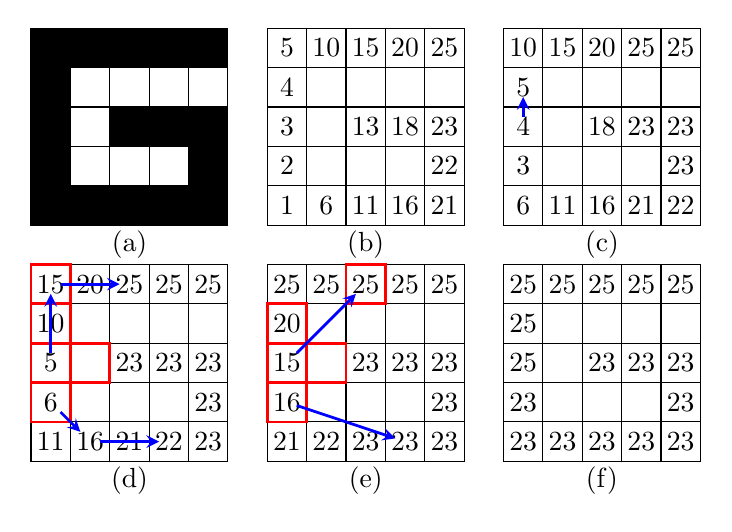
\begin{tikzpicture}[scale=0.5]





\drawgrid{5}{5}

\fillcoord{4}{4}
\fillcoord{3}{4}
\fillcoord{2}{4}
\fillcoord{1}{4}
\fillcoord{0}{4}

\fillcoord{0}{3}
\fillcoord{0}{2}
\fillcoord{0}{1}
\fillcoord{0}{0}

\fillcoord{1}{0}
\fillcoord{2}{0}
\fillcoord{3}{0}
\fillcoord{4}{0}

\fillcoord{4}{1}
\fillcoord{4}{2}

\fillcoord{3}{2}
\fillcoord{2}{2}




\namecoord{2}{-1}{}{(a)}


\drawgrid{5}{5}


\begin{scope}[shift={(6,0)}]
\namecoord{2}{-1}{}{(b)}

\foreach \i in {0,...,4}
\foreach \j in {0,...,4}
{
\namecoord{\i}{\j}{init\i\j}{}
}


\node also [label={[fill=white]center:25}] (init44);
\node also [label={[fill=white]center:20}] (init34);
\node also [label={[fill=white]center:15}] (init24);
\node also [label={[fill=white]center:10}] (init14);
\node also [label={[fill=white]center:5}] (init04);

\node also [label={[fill=white]center:4}] (init03);
\node also [label={[fill=white]center:3}] (init02);
\node also [label={[fill=white]center:2}] (init01);
\node also [label={[fill=white]center:1}] (init00);

\node also [label={[fill=white]center:6}] (init10);
\node also [label={[fill=white]center:11}] (init20);
\node also [label={[fill=white]center:16}] (init30);
\node also [label={[fill=white]center:21}] (init40);

\node also [label={[fill=white]center:22}] (init41);
\node also [label={[fill=white]center:23}] (init42);

\node also [label={[fill=white]center:18}] (init32);
\node also [label={[fill=white]center:13}] (init22);







\drawgrid{5}{5}


\end{scope}

\begin{scope}[shift={(12,0)}]
\namecoord{2}{-1}{}{(c)}

\foreach \i in {0,...,4}
\foreach \j in {0,...,4}
{
\namecoord{\i}{\j}{init\i\j}{}
}


\node also [label={[fill=white]center:25}] (init44);
\node also [label={[fill=white]center:25}] (init34);
\node also [label={[fill=white]center:20}] (init24);
\node also [label={[fill=white]center:15}] (init14);
\node also [label={[fill=white]center:10}] (init04);

\node also [label={[fill=white]center:5}] (init03);
\node also [label={[fill=white]center:4}] (init02);
\node also [label={[fill=white]center:3}] (init01);
\node also [label={[fill=white]center:6}] (init00);

\node also [label={[fill=white]center:11}] (init10);
\node also [label={[fill=white]center:16}] (init20);
\node also [label={[fill=white]center:21}] (init30);
\node also [label={[fill=white]center:22}] (init40);

\node also [label={[fill=white]center:23}] (init41);
\node also [label={[fill=white]center:23}] (init42);

\node also [label={[fill=white]center:23}] (init32);
\node also [label={[fill=white]center:18}] (init22);


\drawgrid{5}{5}


\draw[-stealth,color=blue, line width=1pt] (init02) -- (init03);







\end{scope}

\begin{scope}[shift={(0,-6)}]

\namecoord{2}{-1}{}{(d)}


\foreach \i in {0,...,4}
\foreach \j in {0,...,4}
{
\namecoord{\i}{\j}{init\i\j}{}
}


\node also [label={[fill=white]center:25}] (init44);
\node also [label={[fill=white]center:25}] (init34);
\node also [label={[fill=white]center:25}] (init24);
\node also [label={[fill=white]center:20}] (init14);
\node also [label={[fill=white]center:15}] (init04);

\node also [label={[fill=white]center:10}] (init03);
\node also [label={[fill=white]center:5}] (init02);
\node also [label={[fill=white]center:6}] (init01);
\node also [label={[fill=white]center:11}] (init00);

\node also [label={[fill=white]center:16}] (init10);
\node also [label={[fill=white]center:21}] (init20);
\node also [label={[fill=white]center:22}] (init30);
\node also [label={[fill=white]center:23}] (init40);

\node also [label={[fill=white]center:23}] (init41);
\node also [label={[fill=white]center:23}] (init42);

\node also [label={[fill=white]center:23}] (init32);
\node also [label={[fill=white]center:23}] (init22);


\drawgrid{5}{5}
\selectcoord{1}{2}
\selectcoord{0}{1}
\selectcoord{0}{2}
\selectcoord{0}{3}

\selectcoord{0}{4}

\draw[-stealth,color=blue, line width=1pt] (init02) -- (init04);
\draw[-stealth,color=blue, line width=1pt] (init04) -- (init24);

\draw[-stealth,color=blue, line width=1pt] (init01) -- (init10);
\draw[-stealth,color=blue, line width=1pt] (init10) -- (init30);
% \draw[-stealth,color=blue, line width=1pt] (init03) -- (init14);
% \draw[-stealth,color=blue, line width=1pt] (init04) -- (init24);
\end{scope}


\begin{scope}[shift={(6,-6)}]
\namecoord{2}{-1}{}{(e)}

\foreach \i in {0,...,4}
\foreach \j in {0,...,4}
{
\namecoord{\i}{\j}{init\i\j}{}
}


\node also [label={[fill=white]center:25}] (init44);
\node also [label={[fill=white]center:25}] (init34);
\node also [label={[fill=white]center:25}] (init24);
\node also [label={[fill=white]center:25}] (init14);
\node also [label={[fill=white]center:25}] (init04);

\node also [label={[fill=white]center:20}] (init03);
\node also [label={[fill=white]center:15}] (init02);
\node also [label={[fill=white]center:16}] (init01);
\node also [label={[fill=white]center:21}] (init00);

\node also [label={[fill=white]center:22}] (init10);
\node also [label={[fill=white]center:23}] (init20);
\node also [label={[fill=white]center:23}] (init30);
\node also [label={[fill=white]center:23}] (init40);

\node also [label={[fill=white]center:23}] (init41);
\node also [label={[fill=white]center:23}] (init42);

\node also [label={[fill=white]center:23}] (init32);
\node also [label={[fill=white]center:23}] (init22);


\drawgrid{5}{5}


\selectcoord{1}{2}
\selectcoord{0}{1}
\selectcoord{0}{2}
\selectcoord{0}{3}

\selectcoord{2}{4}

\draw[-stealth,color=blue, line width=1pt] (init02) -- (init24);
\draw[-stealth,color=blue, line width=1pt] (init01) -- (init30);

\end{scope}

\begin{scope}[shift={(12,-6)}]
\namecoord{2}{-1}{}{(f)}

\foreach \i in {0,...,4}
\foreach \j in {0,...,4}
{
\namecoord{\i}{\j}{init\i\j}{}
}


\node also [label={[fill=white]center:25}] (init44);
\node also [label={[fill=white]center:25}] (init34);
\node also [label={[fill=white]center:25}] (init24);
\node also [label={[fill=white]center:25}] (init14);
\node also [label={[fill=white]center:25}] (init04);

\node also [label={[fill=white]center:25}] (init03);
\node also [label={[fill=white]center:25}] (init02);
\node also [label={[fill=white]center:23}] (init01);
\node also [label={[fill=white]center:23}] (init00);

\node also [label={[fill=white]center:23}] (init10);
\node also [label={[fill=white]center:23}] (init20);
\node also [label={[fill=white]center:23}] (init30);
\node also [label={[fill=white]center:23}] (init40);

\node also [label={[fill=white]center:23}] (init41);
\node also [label={[fill=white]center:23}] (init42);

\node also [label={[fill=white]center:23}] (init32);
\node also [label={[fill=white]center:23}] (init22);


\drawgrid{5}{5}



\end{scope}

\end{tikzpicture}



